\chapter{Room 315 Kinematic Transport System}
\label{chap:transport}

Because the available physical parameters were incomplete, I selected a
kinematic rail model and converted the CAD centre-lines into a directed graph.
The resulting controller applies the permitted directions, device behaviour,
spacing and staging logic needed for repeatable routing tests.

I started from project-supplied rail CAD and the physical switch names A1--A4.
I designed the segment vocabulary and topology, then implemented and tested the
dual-rail controller, devices, separation, reservations and staging. No rail
graph or controller was present in the baseline.

\section{Modelling decision: dynamic or kinematic}

I compared a dynamic rigid-body model driven by wheel--rail contact with a
kinematic model that places each shuttle from its graph segment and travelled
distance. Dynamic simulation would suit traction, slip or wear studies, but a
credible eight-shuttle model required unavailable mass, friction, compliance,
drive and switch data; apparent physical accuracy would therefore be
unsupported. The project instead needed repeatable routing, sensor crossings,
arrivals, camera scenes and supervised execution. I selected kinematic motion
because it isolates geometry, topology and authorisation while producing those
observations consistently. It does not claim wheel--rail dynamics.

\section{Kinematic transport backend}

The backend advances arc length on the calibrated graph and publishes poses
through Gazebo's \code{set\_pose} service. Gravity and wheel contact do not drive
the shuttle; controller state is authoritative, so rendering lag does not alter
logical progression.

Before detailing the graph, \cref{fig:rail-reality-gazebo} relates each physical
transport cell to its integrated Gazebo counterpart. The views provide an
orientation aid and a qualitative assembly check; the following sections give
the calibrated geometry, topology and behavioural evidence.

\begin{figure}[p]
  \centering
  \captionsetup{skip=4pt}
  
\includegraphics[width=0.92\textwidth,trim=39bp 99bp 39bp 43bp,clip]
  {reality_to_simulation/rail_right.png}
  \par\vspace{1mm}
  
\includegraphics[width=0.92\textwidth,trim=33bp 63bp 34bp 105bp,clip]
  {reality_to_simulation/rail_left.png}
  \caption[Physical-to-Gazebo comparison of the two Room~315 rail cells.]
  {Physical-to-Gazebo comparison of the two Room~315 transport cells: the
  right rail is shown above and the left rail below. The differing viewpoints
  make this a qualitative check of the loop and branch layouts.}
  \label{fig:rail-reality-gazebo}
\end{figure}

\section{From SolidWorks points to a continuous rail graph}

SolidWorks is a three-dimensional CAD application
\citep{solidworks3dcad}. I used it to inspect the project-supplied rail model
and export its centre-line points. Both rail configurations use the resulting
276 ordered points in 14 CSV curves. I split them at branch boundaries,
preserved their direction, mapped each public segment to a curve and applied
side-specific calibration before Gazebo publication. CSV files define
\emph{geometry}; YAML successor rules define \emph{connectivity}.

Each public segment has an arc length and the normalised coordinate
\(\rho=s/L\) from \cref{eq:sratio}; the public interface names this value
\code{s\_ratio}. Cubic Hermite interpolation was retained
because it joins samples with continuous heading; linear interpolation produced
yaw jumps, while an unconstrained global spline could leave the rail. Tests
compared the runtime evaluator with the source polyline and checked route and
device mappings. \Cref{fig:rail-geometry-source} shows the configured
reconstruction; the data schema, transform and evaluator details are in
\cref{app:technical}.

\begin{figure}[H]
  \centering
  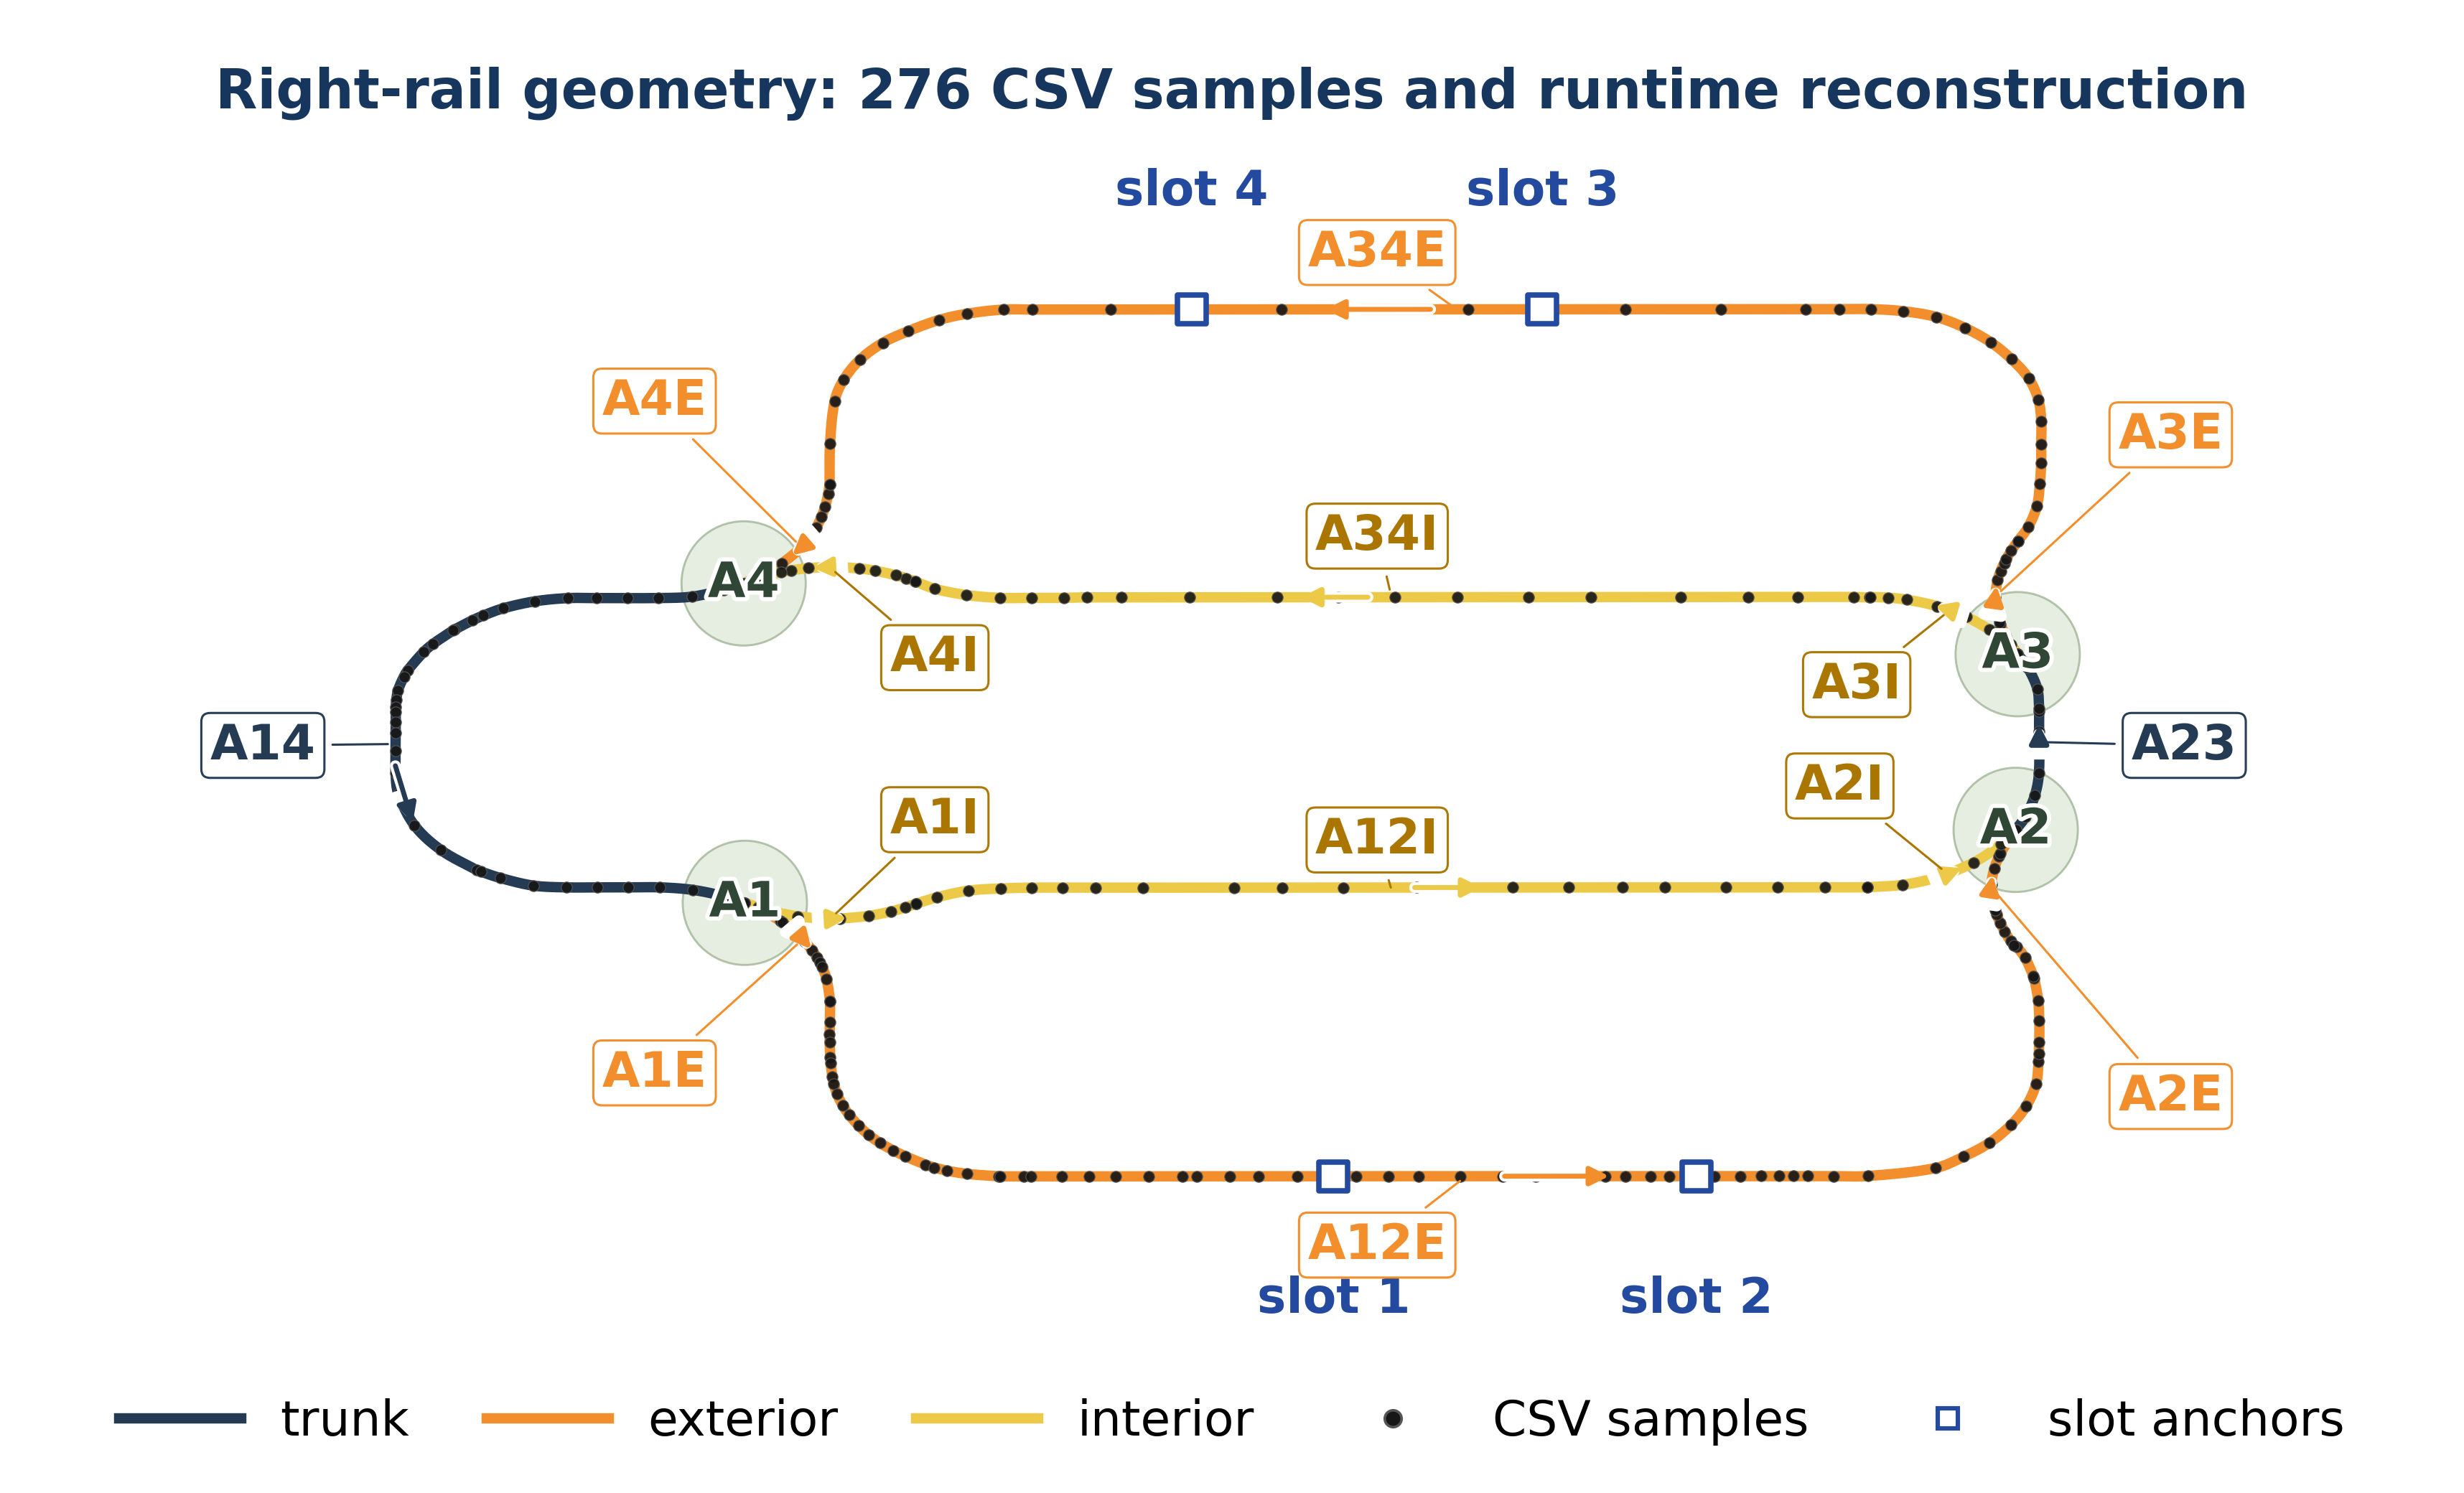
\includegraphics[width=0.98\textwidth]{figures/f07_calibrated_rail_geometry_current.png}
  \caption[Ordered CSV source points and current Hermite rail geometry.]
  {Room~315 centre-line from 276 ordered CAD/CSV samples: black dots are source
  points and coloured curves are dense Hermite outputs. The drawing shows the
  right-rail source/CAD orientation; the left rail reuses the samples with its
  own internal geometry identifiers and calibration. Affine calibration applies
  side-specific planar scale, rotation and translation plus height/yaw offsets before Gazebo
  publication. This checks the configured reconstruction; no independent
  metrology was available.}
  \label{fig:rail-geometry-source}
\end{figure}

\section{Topology, inherited switch names and segment vocabulary}

The physical installation and project documentation already identified the
four switch devices/zones as A1--A4; I retained these inherited identifiers.
They name switches, not rail segments. Starting from them, I designed the
14-label public segment vocabulary shared by the controller, ROS~2 interfaces,
visual labels and PDDL model.

In this convention, \code{E} means exterior and \code{I} means interior (the
inner branch). A one-number form \code{AiE}/\code{AiI} denotes the short
connector adjacent to switch Ai. A two-number form
\code{AijE}/\code{AijI} denotes the exterior/interior route between switch
zones Ai and Aj; for example, \code{A34E} is the exterior A3--A4 segment between
the adjacent connectors \code{A3E} and \code{A4E}, while \code{A12I} is the
interior A1--A2 segment. An unsuffixed two-number form is a shared single-track
section, such as \code{A23} or \code{A14}.

When switch selections are consistent, the directed segment sequence is
\[
\texttt{A14} \rightarrow \texttt{A1E/I} \rightarrow \texttt{A12E/I}
\rightarrow \texttt{A2E/I} \rightarrow \texttt{A23} \rightarrow
\texttt{A3E/I} \rightarrow \texttt{A34E/I} \rightarrow
\texttt{A4E/I} \rightarrow \texttt{A14}.
\]
These labels and successor rules form the discrete topological language of my
hybrid routing design; position within a segment remains continuous through arc
length \(s\). They are software interface states, not additional physical rails.
Each shuttle moves only in the forward direction shown by the arrows; reverse
travel is outside the controller and planning contracts.

Each switch has exactly two positions, \code{EXTERIOR} and \code{INTERIOR}.
With four switches per rail, this gives \(2^4=16\) assignments. The left/right
network YAML files define the nodes, 14 segments, connections and
switch-conditioned successors.

The controller and PDDL generator read this same public topology on both rails;
left-side internal geometry names are normalised before publication. Rules,
rather than point distance, select the successors listed in
\cref{tab:rail-topology}. In forward traversal A2 enters \code{A23}, then A3
selects its exterior/interior successor.

\begin{table}[H]
\centering
\footnotesize
\renewcommand{\arraystretch}{1.00}
\caption{Successor map for the public segment vocabulary shared by both rails.}
\label{tab:rail-topology}
\begin{minipage}[t]{0.485\textwidth}
\centering
\setlength{\tabcolsep}{2.4pt}
\begin{tabular}{@{}llll@{}}
\toprule
\textbf{Segment} & \textbf{Switch} & \textbf{State} & \textbf{Next}\\
\midrule
\code{A23}  & \code{A3} & \code{E} & \code{A3E}\\
\code{A23}  & \code{A3} & \code{I} & \code{A3I}\\
\code{A3E}  & ---        & Any       & \code{A34E}\\
\code{A3I}  & ---        & Any       & \code{A34I}\\
\code{A34E} & \code{A4} & \code{E} & \code{A4E}\\
\code{A34E} & \code{A4} & \code{I} & \code{FALLING}\\
\code{A34I} & \code{A4} & \code{E} & \code{FALLING}\\
\code{A34I} & \code{A4} & \code{I} & \code{A4I}\\
\code{A4E}  & ---        & Any       & \code{A14}\\
\code{A4I}  & ---        & Any       & \code{A14}\\
\bottomrule
\end{tabular}
\end{minipage}\hfill
\begin{minipage}[t]{0.485\textwidth}
\centering
\setlength{\tabcolsep}{2.4pt}
\begin{tabular}{@{}llll@{}}
\toprule
\textbf{Segment} & \textbf{Switch} & \textbf{State} & \textbf{Next}\\
\midrule
\code{A14}  & \code{A1} & \code{E} & \code{A1E}\\
\code{A14}  & \code{A1} & \code{I} & \code{A1I}\\
\code{A1E}  & ---        & Any       & \code{A12E}\\
\code{A1I}  & ---        & Any       & \code{A12I}\\
\code{A12E} & \code{A2} & \code{E} & \code{A2E}\\
\code{A12E} & \code{A2} & \code{I} & \code{FALLING}\\
\code{A12I} & \code{A2} & \code{E} & \code{FALLING}\\
\code{A12I} & \code{A2} & \code{I} & \code{A2I}\\
\code{A2E}  & ---        & Any       & \code{A23}\\
\code{A2I}  & ---        & Any       & \code{A23}\\
\bottomrule
\end{tabular}
\end{minipage}
\end{table}

Here, ``Any'' denotes an unconditional successor. An incompatible converging
switch has no successor and enters \code{FALLING}: a latched
no-valid-successor fault that stops at the segment end, not a physical fall.

\section{Devices and their public identifiers}

Switches A1--A4 select exterior or interior branches and report their state;
stoppers hold or release approaching shuttles; binary sensors report occupancy
and shuttle identity. DZI identifiers denote indexed slot detectors, while DA
identifiers denote switch-approach or branch detectors. The target workflow
prepares the stopper, requests motion and waits for the identity-bearing DZI;
continuous controller pose is not a learned-model input. Exact names, states,
protected distances and the device map are in \cref{app:technical};
\cref{chap:interfaces} defines the supervisory vetoes.

\section{Multi-shuttle identity and lifecycle}

Each rail supports four stable identities: L1--L4 or R1--R4, mapped to Gazebo
entities and never inferred from array order. The registry keeps configuration,
world entities, controller reports, vision and planner objects aligned. It
supports per-shuttle enable, disable, reset and removal, while emergency stop
disables the fleet until an explicit resumption decision. Only the eight
language-interface identities enter supervised execution; detailed service and
mode values are in \cref{app:technical}.
\Cref{fig:dense-eight-shuttle} shows the full fleet in both visual-pipeline
cameras.

\begin{figure}[htbp]
  \centering
  \begin{subfigure}[t]{0.49\textwidth}
    \centering
    
\includegraphics[width=\linewidth]{f07_dense_left_camera.png}
    \caption{Left: L1--L4; L2 and L4 loaded.}
  \end{subfigure}
  \hfill
  \begin{subfigure}[t]{0.49\textwidth}
    \centering
    
\includegraphics[width=\linewidth]{f07_dense_right_camera.png}
    \caption{Right: R1--R4; R1 and R3 loaded.}
  \end{subfigure}
  \caption[Paired Gazebo camera views of the complete eight-shuttle fleet.]
  {Synchronous overhead Gazebo views of all eight shuttles. With device markers
  hidden, identity colours, presence and payload appearance remain visible.}
  \label{fig:dense-eight-shuttle}
\end{figure}

\section{Motion, slots and occupancy}

At every update step, an enabled shuttle advances by
\begin{equation}
  s_{k+1}=s_k + v\,\Delta t ,
  \label{eq:kinematic-update}
\end{equation}
where \(s_k\) is arc length at update \(k\), \(v\) configured forward speed and
\(\Delta t\) the interval. Route, target, stopper and headway constrain the
update; crossing an end transfers residual distance to the topology-selected
successor. Timing details are in \cref{app:technical}.

Slots are calibrated exterior-segment \code{s\_ratio} values. Arrival combines
target, stopper, slot detector and OFF command effect: OFF reports DISABLED,
while \code{reached\_target\_slot} records low-level setpoint completion, not
task success. The planner tracks symbolic occupancy; the executive still
verifies target identity.

\section{Operator-facing observation and maintenance}

The low-level API supports commissioning without bypassing supervised task
execution. Its device-position tool projects a Gazebo point onto configured rail
geometry, defaults to a non-writing preview and guards large-residual updates;
changes take effect only after relaunch and feedback checking. Commands and
maintenance procedures are listed in \cref{app:technical} and the runbook.

\section{Headway and collision constraints}

The controller enforces a configurable default \SI{0.33}{m} centre separation.
This is a kinematic anti-overlap constraint, not a measured braking or machinery
safety distance. Higher-level
headway and reservations require clear route blocks ahead
(\cref{chap:interfaces}). A \emph{blocker} is another shuttle occupying the
route, destination or holding capacity; other objects are outside this model.

\section{Interior staging and dense blocker cases}

Interior branches \code{A12I}/\code{A34I} are capacity-limited holding areas;
their calibrated length, margins and separation admit at most two shuttles.
Successful staging records a clearance certificate linking identity, bounded
motion, stop and post-stop observation. It supports route normalisation rather
than visual localisation and is invalidated by later motion;
\cref{chap:neurosymbolic} covers recovery and \cref{app:technical} the exact
fields.

\section{Conclusion}

The result is repeatable motion on two calibrated rail graphs with stable
shuttle identity and device feedback. All 96 transport checks passed across
geometry, connections, devices, minimum spacing and route ownership
(\cref{chap:results}), and the integrated campaign exercised blocked routes.
The central difficulty was converting sampled CAD curves and one-way switch
behaviour into one route map.
